\documentclass[12pt]{article}

\usepackage[bottom = 15mm]{geometry}
\usepackage[utf8]{inputenc}
\usepackage[T2A]{fontenc}
\usepackage[russian]{babel}
\usepackage{graphicx}
\usepackage{caption}
\usepackage{amssymb, gensymb, amsmath}
\usepackage{mathrsfs}
\usepackage{array, colortbl}


\textwidth = 16 cm
\textheight = 23  cm
\oddsidemargin = 0 pt
\topmargin = -1.5 cm
\parindent = 20 pt
\parskip = 0 pt
\flushbottom


\title{{\bf Задача 3.\,2.\,5 \\ Вынужденные колебания в электрическом контуре}}
\author{Лось Денис (группа 611)}
\date{9 ноября 2017}



\begin{document}

\maketitle

\paragraph{Цель работы:} исследование вынужденных колебаний и процессов их установления.

\paragraph{В работе используются: } генератор звуковой частоты, осциллограф, вольтметр, частотометр, ёмкость, индуктивность, магазин сопротивлений, универсальный мост.

\section*{Экспериментальная установка}
\par	
	Для экспементального исследования резонансной кривой тока в последовательном колебательном контуре можно снять зависимость амплитуды напряжения на резисторе $R$ от частоты генератора (при постоянной амплитуде выходного напряжения на генераторе). Однако импеданс этого контура будет включать в себя также выходной импеданс генератора. Нам следует убедиться, что выходной импеданс генератора много меньше импеданса контура и не влияет на процессы, происходящие в контуре.
\par	
	Чтобы устранить влияние импеданса генератора, можно использовать принципиальную схему, изображённую на рис.1: синусоидальный сигнал с генератора подаётся на параллельный колебательный контур через небольшую разделительную ёмкость $C_1$.
\begin{figure}[h!]
	\centering
	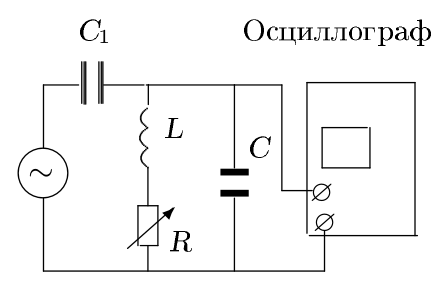
\includegraphics[width = 7 cm, height = 4 cm]{image1.png}
	\caption{Принципиальная схема установки для исследования вынужденных колебаний}
\end{figure}
\newpage
\par	
	Зависимость амплитуды этого напряжения от частоты генератора будет практически совпадать с резонансной кривой для последовательного контура, если импедансы возбуждающей и измеряющей цепей намного превосходят импеданс самого контура вблизи резонанса $Z_\text{рез} = L / \left( R C \right) = Q / \left(\Omega C \right)$. Разделительная ёмкость $C_1$ выбирается настолько малой, что в рабочем диапазоне частот её импеданс $Z_\text{$C_1$} = 1 / \left( \Omega C_1 \right)$ много больше импеданса контура, поэтому в цепи генератора течёт ток практически с постоянной амплитудой, а колебательный контур выполняет роль нагрузочного сопротивления, которое, в свою очередь, зависит от частоты. Поскольку в резонансе сопротивление $Z_\text{рез}$ параллельного контура максимально, то и напряжение на ёмкости $C$ тоже маскимально. Входное сопротивление осциллографа должно быть достаточно велико $R_\text{эо} = 1 \, \text{МОм}$.
\par
	Таким образом, при выполнении условий
\begin{equation}
	Z_\text{$C_1$} = \frac{1}{\Omega C_1} \gg |Z_\text{рез}| = \frac{Q}{\Omega C}, \quad R_\text{эо} \gg \frac{Q}{\Omega C} \notag
\end{equation}
и при условии, что действительная часть импеданса катушки много меньше её мнимой части, резонансная кривая в нашем контуре будет выглядить так же, как и в последовательном: максимум амплитуды при резонансе.
	Схема экспериментальной установки для исследования вынужденных колебаний приведена на рис.2.
\begin{figure}[h!]
	\centering
	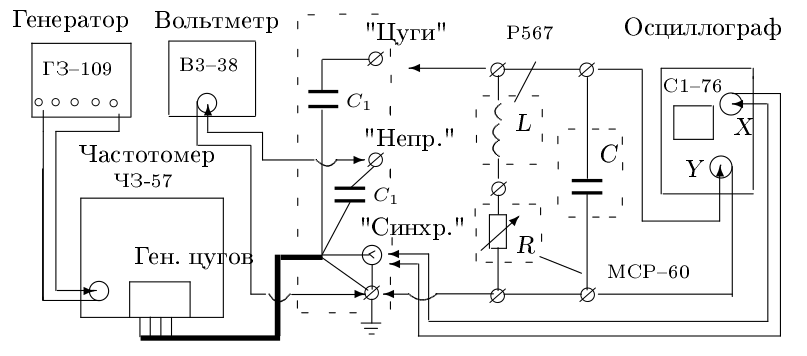
\includegraphics[width = 12 cm, height = 6.5 cm]{image2.png}
	\caption{Схема экспериментальной установки для исследования вынужденных колебаний}
\end{figure}
\section*{Ход работы}
\subsection*{Исследование резонансных кривых}
	\par
		Соберём схему согласно рис.2, установив на магазине индуктивностей значение $L = 100$ мГн, а на магазине сопротивлений $R = 0$ Ом. В данной экспериментальной установке $C = 0.1 \, \text{мкФ} \, \left(\sigma_C = 2 \% \right)$. Рассчитаем теоритическую резонансную частоту контура $f_\text{теор} = 1 \, / \left(2 \pi \sqrt{LC} \right)$. Получим, что теоритическая резонансная частота контура $f_\text{теор} = 1591$ Гц. Найдём экспериментальную резонансную частоту, получим, что $f_0 = 1550 $ Гц.
	\par
		Меняя частоту генератора в  обе стороны от резонансной, снимем зависимость показаний вольтметра $U$ от показаний частотометра $f$. По окончании измерений установим на магазине сопротивлений значение $R = 100$ Ом и повторим измерения. Затем построим на одном графике резонансные кривые в координатах $U / U_0 = G(f / f_0)$, где $U_0$ --- напряжение при резонансной частоте $f_0$ Гц.		
	\begin{table}[h!]
		\centering
		\begin{tabular}{|c|c|c|c|c|c|c|c|c|c|c|c|c|}
		\hline
		$U$, В & 5.70 & 6.33 & 6.96 & 7.28 & 7.91 & 8.54 & 8.23 & 7.59 & 6.96 & 6.65 & 6.33 &  5.70 \\
		\hline
		$f$, Гц & 1519 & 1525 & 1530 & 1532 & 1537 & 1542 & 1563 & 1568 & 1572 & 1575 & 1578 & 1583 \\
		\hline
		\end{tabular}
		\caption{Зависимость $U = G(f)$ при $R = 0$ Ом и $U_0 = 9.02$ В}		
	\end{table}
	\begin{table}[h!]
		\centering
		\begin{tabular}{|c|c|c|c|c|c|c|c|c|c|c|}
		\hline
		$U$, В & 1.42 & 1.58 & 1.74 & 1.90 & 2.06 & 2.06 & 1.90 & 1.74 & 1.58 & 1.42 \\
		\hline
		$f$, Гц & 1447 & 1463 & 1481 & 1501 & 1518 & 1601 & 1623 & 1648 & 1672 & 1703 \\
		\hline
		\end{tabular}
		\caption{Зависимость $U = G(f)$ при $R = 100$ Ом и $U_0 = 2.22$ В }		
	\end{table}	
	\begin{figure}[h!]
		\centering
		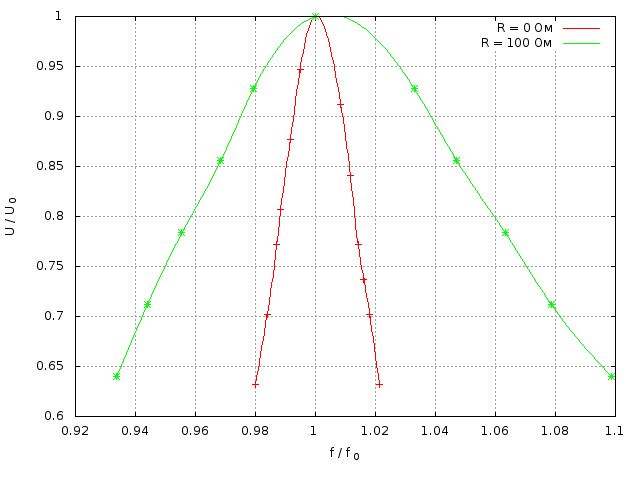
\includegraphics[height = 8cm, width = 14 cm]{plot1.png}
		\caption{Резонансные кривые для $R = 0$ Ом и $R = 100$ Ом}
	\end{figure}	
	\par
		Найдём добротность контура при $R = 0$ Ом и $R = 100$ Ом как $f_0 \, / \left(2 \, \Delta f_\text{$0.7$} \right)$. Получим, что
		\begin{align*}
			Q_0 &= \left(29 \pm 1 \right) \\
			Q_\text{$100$} &= \left(7.40 \pm 0.04 \right)
		\end{align*}
	\newpage
\subsection*{Процессы установления и затухания колебаний}
\par	
	Подключим контур к клемме Цуги и установим на генераторе резонансную частоту. В данном случае экспериментальная резонансная частота $f_\text{0 эксп.} = 1603$ Гц. Убедимся, что огибающая затухающих колебаний --- это перевёрнутая огибаюзая нарастающего участка.
\par
	Для рассчёта добротности по скорости нарастания и скорости затухания будем измерять амплитуды двух колебаний $U_k$ и $U_\text{$k + n$}$, разделённых целым числом периодов $n$, а также амплитуду установившихся колебаний $U_0$ в случае нарастания. Проведём измерения при $R = 0$ Ом и $R = 100$ Ом. Для расчёта по нарастанию амплитуды получим, что $U_0 = 2.8$ дел и $U_0 = 0.8$ дел при $R = 0$ Ом и $R = 100$ Ом соотвественно.
\begin{table}[h!]
	\centering
	\begin{tabular}{|c|c|c|c|c|c|c|}
	\hline
	$R$, Ом & \multicolumn{4}{|c|}{0} & \multicolumn{2}{|c|}{100} \\
	\hline
	$U_k$, дел & 1.6 & 0.8 & 1.6 & 1.6 & 0.2 & 0.2 \\
	\hline
	$U_\text{$k+n$}$, дел & 2.2 & 1.6 & 1.8 & 2.0 & 0.4 & 0.6 \\
	\hline
	$n_T$ & 6 & 4 & 1 & 3 & 1 & 2\\  
	\hline
	$Q$ & 27.19 & 24.60 & 17.23 & 23.24 & 7.75 & 5.72\\
	\hline
	\end{tabular}
	\caption{Измерения $U_k$ и $U_\text{$k+n$}$ для расчёта добротности по нарастанию амплитуды}
\end{table}
\par			
	В данном случае (при расчёте добротности по нарастанию амплитуды) мы определяем добротность $Q$ как $\pi / \Theta $, где логарифмический декремент затухания
	\[
		\Theta = \frac{1}{n} \, \ln{\frac{U_0 - U_k}{U_0 - U_\text{$k+n$}}}
	\]	
\begin{table}[h!]
	\centering
	\begin{tabular}{|c|c|c|}
	\hline
	$R$, Ом & 0 & 100 \\
	\hline
	$U_k$, дел & 1.2 & 0.6 \\
	\hline
	$U_\text{$k+n$}$, дел & 0.8 & 0.4 \\
	\hline
	$n_T$ & 3 & 1\\  
	\hline
	$Q$ & 23.23 & 7.74\\
	\hline
	\end{tabular}
	\caption{Измерения $U_k$ и $U_\text{$k+n$}$ для расчёта добротности по затуханию амплитуды}
\end{table}
\par
	Измерим активное сопротивление $R_L$ и индуктивность $L$ магазина индуктивностей с помощью измерителя $LCR$ на частотах 50 Гц, 500 Гц, 1500 Гц.
\begin{table}[h!]
	\centering
	\begin{tabular}{|c|c|c|}
	\hline
	$f$, Гц & $R$, Ом & $L$, мГн \\
	\hline
	50 & 28.98 & 99.924 \\
	\hline
	500 & 29.20 & 99.912 \\
	\hline
	1500 & 30.37 & 99.932 \\	
	\hline
	\end{tabular}	
\end{table}
\newpage
\par
Теоритические значения добротности мы можем найти как $1 / R \cdot \sqrt{L / C}$. В результате получим, что
		\begin{align*}
			Q_\text{0 теор.} &= 33  \\
			Q_\text{100 теор.} &= 7.67 \\
		\end{align*}
	Сместим частоту генератора с резонансного значения и получим на экране картину биений. Полученная таким образом картина:
\begin{figure}[h!]
	\centering
	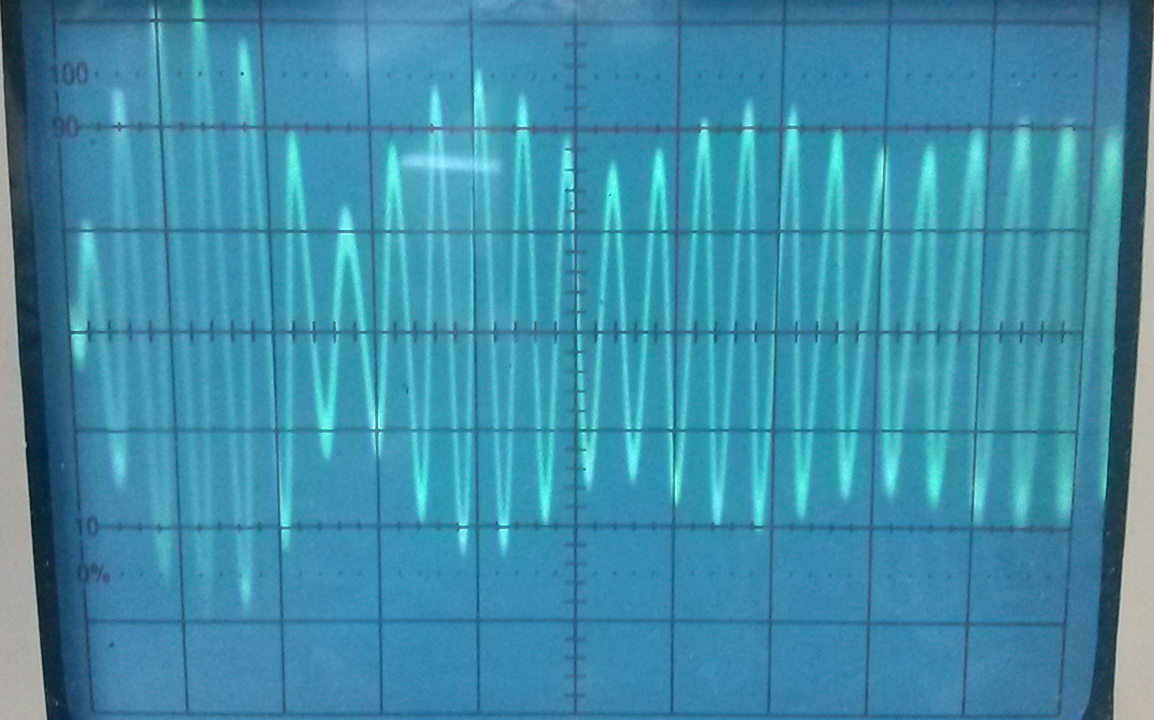
\includegraphics[width = 12cm, height = 6cm]{image3.png}
	\caption{Наблюдаемая картина биений}
\end{figure}	 					

\end{document}